\documentclass[letterpaper, 10 pt, conference]{ieeeconf}

\usepackage{algorithm}
\usepackage[noend]{algpseudocode}
\usepackage{bm}

\usepackage{amsfonts}
\usepackage[pdftex]{graphicx}
\usepackage{comment}

\usepackage{caption}
\usepackage{subcaption}

%\usepackage{amsthm}
\newtheorem{thm}{Theorem}
\newtheorem{lem}{Lemma}
%\newtheorem{asmp}{Assumption}
\newtheorem{defn}{Definition}
%\newtheorem{clm}{Claim}

\IEEEoverridecommandlockouts                              % This command is only needed if 
                                                          % you want to use the \thanks command

\overrideIEEEmargins                                      % Needed to meet printer requirements.

\title{\LARGE \bf
Homotopy-Aware RRT$^{*}$ : Toward Human-Robot Topological Path-Planning
}

\author{
Daqing Yi, Michael A. Goodrich and Kevin D. Seppi
\thanks{Daqing Yi, Michael A. Goodrich and Kevin D. Seppi are with Department of Computer Science, Brigham Young University, Provo, UT, 84604, USA.
{\tt\small daqing.yi@byu.edu, mike@cs.byu.edu, kseppi@cs.byu.edu} }
}

\begin{document}


\maketitle
\thispagestyle{empty}
\pagestyle{empty}


%%%%%%%%%%%%%%%%%%%%%%%%%%%%%%%%%%%%%%%%%%%%%%%%%%%%%%%%%%%%%%%%%%%%%%%%%%%%%%%%
\begin{abstract}
Many researchers have noted that humans often represent the world using a topological rather than metric-based path-planning~\cite{kuipers99,aginsky1997two}, and various methods have been used to create topological-representations that can be used by path-planners for robots~\cite{mataric1992integration,thrun1998learning,fasola2013modeling,shah2013qualitative}.  
The idea of these planners is often to create algorithms that blend the benefits of graph-based path planners with the postulated topological representations used by a human partner or supervisor.
Such planners can produce paths consistent with well-reasoned topologies, but the planners may not work well in worlds that have sparse features or when the human intends a topological reference to be a ``soft'' constraint rather than a rigid path requirement. 
In this paper, we propose HA-RRT$^{*}$, a homotopy-aware RRT$^{*}$, that explores the planning space for optimal solutions while respecting the path topology.
The paper restricts attention to problems where the goal is not only to optimize some objective but also contains ``soft'' or ``hard'' topological constraints, i.e. ``go quickly from A to B avoiding C''.
Because the algorithm is aware of the homotopy class of each branch of the tree produced by the RRT algorithm, the algoirthm can enable type of sliding autonomy for different levels of human's intent on the path topology.
Thus, a clear intent on the path topology provides the homotopic constraint, which reduces the working space of the optimal search; a vague intent on the path topology can be identified by comparing the optimal solutions in different homotopy classes.
The paper includes a set of simulation case studies and a corresponding theoretic analysis.
\end{abstract}

\begin{comment}
six pages
\end{comment}

%%%%%%%%%%%%%%%%%%%%%%%%%%%%%%%%%%%%%%%%%%%%%%%%%%%%%%%%%%%%%%%%%%%%%%%%%%%%%%%%
\section{Introduction}
\label{sec:intro}

An optimization problem is usually formed by a human who specifies a metric that attempts to encode task performance in a numerically amenable form.
As the task supervisor, the so-called {\em problem holder} in Woods' nomenclature~\cite{woods2004envisioning}, it is essential that the human's intent is correctly and precisely modeled.
%Optimality has been the most important heuristic in planning motions for the robots.
In planning a robot's motion for a task, the most common ways to model intent is with single numerical objective~\cite{6974170} or with multiple numerical objectives~\cite{yi2014supporting}.  Examples of objectives are many: Euclidean distance, minimum time, etc.
A numerical solver is then used to generate a path that optimizes the given objectives.

Unfortunately, not all types of human intent can be easily modeled using common measurable objectives.
One difficult-to-model intent is the ``shape'' of the planned path.  Although shape properties like continuity and smoothness can be modeled using standard numerical constraints, shapes that refer to environment topology, such as ``go around building A and then between the two trees while avoiding region C,'' benefit from topological approaches.  In particular, concepts from algebraic topology can be used to create numerical representations of these topological desiderata or constraints.  In this paper, we present an algorithm that allows the human to specify avoiding regions, moving around objects, and satisfying constraints: via-point/waypoint constraints, reference path constraints~\cite{6974170} and temporal logic constraints~\cite{5650896}.
%This method won't work when there is only preference on the ``shape'' of the paths instead of hard constraint.
%At the same time, the preference on the ``shape'' of the paths might also be fuzzy for the human to describe.

The topological concept of \emph{homotopy} is a mathematical formalism of the inherent similarity or dissimilarity of two paths.
Given two paths, if one can be deformed into the other without encroaching any obstacle, they are said to be \emph{homotopic}~\cite{Hernandez201544}.
The set of paths that are homotopic to each other form a \emph{homotopy class}, and the  set of homotopy classes partition the set of all possible paths between any two points $A$ and $B$.
In an environment containing obstacles, the homotopy partition can provide a useful way of grouping paths together based on the similarities of their ``shapes," where the term ``shape'' is interpreted using the formal topological notion.
%{\sc Walter, I think we actually use a slightly different partitioning of the space.  The first difference is that we are using homologies instead of homotopies.  This is a technical difference that shouldn't make much difference, but we should point out to the reader that we are aware of this difference.  The second difference is that we don't actually partition the set of possible paths.  Instead, we partition the 2-D space of the environment.  The partition of the environment space is motivated by a desire to group paths through that space into intuitive groups based on topological properties, and this is an important distinction.}

%{\sc Fundamental (algebraic) group of topology. How our approach isn't about arbitrarily complex paths within a homotopic class, but rather has some ``natural'' boundaries in metric space.  
%How this lends itself to efficient RRT*.  
%How this differs from Vijay's homotopy-based path planning.  Homology or homotopy?}

%{\it In Vijay's paper, the map is discretized to graph, and then calculating the complex values of each edge. The complex value tells whether two paths are in same homotopy class. Ours follows another approach, which is sampling based. While exploring, we can tell if the current sub-path can still lead to a path that belongs to some homotopy class. That is why it is called homotopy aware. 

%When we have the homotopy class as constraint, it can be used to reduce the exploring region so that the efficiency can be improved.
%Because a branch of the tree will not be extended if it leads to a region that is not satisfied by the homotopic constraint.}

Importantly, simple representative paths from within a homotopy class can often be associated with human intent.
Consider a path-planning problem where a human supervisor defines the task for a robot.  Further, consider the following list of ways in which a human can express intent about path shape, and the corresponding homotopy-based constraint:
%The task is needed to be modeled so that the robot can understand and plan for execution.
%Let the objective be only reaching to a target quickly, there can be several levels of how clear his intent is.
\begin{enumerate}
\item \emph{I want the path to visit a sequence of specific regions.}
Topologically, such a path is constrained to one homotopy class, so this homotopy class becomes the constraint of the optimization problem~\cite{Hershberger199463}.
%This homotopy class could be defined from a human initialized reference path.
\item \emph{I want the path to visit some regions and avoid other regions.}
Since it is possible that several homotopy classes can satisfy these requirements, the homotopic constraint restricts the path to  the set of homotopy classes that satisfy the requirements.
\end{enumerate}
The first two ways of expressing human intent translate into homotopic path constraints.  The next two allow a human to express preference among different path shapes, but also allow the human to tradeoff between following a desired path shape and optimizing another performance objective.
\begin{enumerate}
\setcounter{enumi}{2}
\item \emph{I prefer some path shapes over others, but I recognize that tradeoffs may be needed.} 
This indicates that the human has preferences over different homotopy classes, but also acknowledges that certain homotopy classes may not allow an acceptable optimization of another task-based objective.
If the preference on the homotopy classes can be modeled using an objective function, then non-dominant solutions over the task-based objective and homotopic objective can be found, and the human can select one of these solutions.
\item \emph{I have preferences over paths but it need help in understanding these preferences.}
In this case, the human's preference could be identified through interactive process.
Another straightforward way is that the planning algorithm provides the best solution of each homotopy class to the supervisor.
The supervisor can then select one that satisfy his/her intent.
\end{enumerate}

In order to support these forms of human intent, expressed as homotopic constraints and preferences, we propose a homotopy-aware RRT$^{*}$ (HA-RRT) algorithm.  This algorithm uses an RRT$^*$ algorithm to explore possible paths, but each branch of the random tree is aware of the homotopy class to which it belongs.  The remainder of the paper presents this algorithm. We first review the relevant work in section~\ref{sec:related_work}.
We then introduce the algorithm in section~\ref{sec:algorithm} and show how it can be used to implement the different forms of human intent in section~\ref{sec:application}. An analysis of the algorithm is given in section~\ref{sec:analysis}, and then conclusions are presented.

\section{Related work}
\label{sec:related_work}

Humans often represent the world using a topological rather than metric-based path-planning~\cite{kuipers99,aginsky1997two}, and various methods have been used to create topological-representations that can be used by path-planners for robots~\cite{mataric1992integration,thrun1998learning,fasola2013modeling,shah2013qualitative}.  
The topological notion of homotopy presents a formal definition of the similarity between two paths.
This definition can be used both to determine the similarity between two paths as well as to partition paths into different classes.
Homotopy-based path planning requires an algorithm to determine the homotopic equivalence of two paths, which is usually computationally expensive.

{\sc rewrite the following three paragraphs -- there are English language issues.}

A Voronoi diagram-based algorithm has been used to determine homotopy classes, but this algorithm shows limitations on finding some paths in some cases~\cite{banerjee2013framework}.
%Specifically, generating Voronoi diagram for obstacles of complicated shapes is hard.
By algebraic topology, the path of same homotopy class can be determined by using orientable band~\cite{Hershberger199463}.
Similarly, the complexity of the problem is increased when the shapes of the obstacles are not smooth and convex.
Semi-algebraic cuts are used to converting the path into ``word'' so that the homotopic equivalence can be compared~\cite{Grigoriev:1998:PAS:281508.281528}.
The Cauchy Integral theorem has been introduced to determine homotopy class by marking the positions in the obstacles as undefined~\cite{AAAI101920}.
Given two paths sharing the same start and goal, we can determine whether there is an obstacle inside the region that the two paths close by the value of the complex integral.
Because the map is discretized, the computation cost expands greatly if the obstacles are reasonably approximated by the cells.

Sampling-based path planning, like RRT or PRM, has been an effective and popular tool of generating planning paths.
The idea of homotopy has also been integrated as well.
By homotopic redundancy, the paths from PRM could be compared by the homotopy classes~\cite{1041613}.
By dividing the space using the rays crossing each obstacle, reference frames could be used to represent the paths into canonical sequences~\cite{Hernandez201544}.
In this way, the extending process of the graph structure keeps tracking the homotopy class of the new branch so that the exploration process can be constrained in some homotopy classes.

In order to accelerate the exploration process, bidirectional RRT has been introduced to accelerate the exploration process.
The bidirectional exploration reserves the optimality in the optimal sampling process
~\cite{Jordan.Perez.ea:CSAIL13}~\cite{starek2014bidirectional}.
With two trees exploring from two directions, we can have the optimal cost-to-go and the optimal cost-to-arrive at different position.
This guarantee the optimality search with the homotopic constraint.
We introduce the homotopy-aware bidirectional RRT$^{*}$ to support different level of intent on topology for the task supervisor.

\section{Homotopy-aware RRT$^{*}$}
\label{sec:algorithm}

%Without loss of generality, we only look at the minimization problem of the path planning.
Definition \ref{def:homo_path_planning} presents the homotopy-based optimal path-planning problem formed as a minimization problem.
%It can be extended into other homotopy-relevant optimal path planning.
\begin{defn}{ \textbf{Homotopy-Based Optimal Path-Planning} }
\label{def:homo_path_planning}
Consider a bounded, connected open set $ X \subset \mathbb{R}^{d} $, an obstacle space $ X_{\it obs} $, an initial state $ x_{init} $, and a goal state $ x_{goal} $. 
Denote the obstacle-free space by $ X_{\it free} = X \setminus X_{\it obs} $.
Define a {\em path} in $X$ as a continuous curve parameterized by $s$, denoted by $\sigma : [0,s] \rightarrow X$. 
Define the cost of the path as $ \mbox{\sc Cost} (\sigma) $.  
The goal is to find paths $ \sigma^{*} \in \Sigma^{*}$ such that
\textit{ (a) } $ \forall \tau\in[0,s], \sigma^*(\tau) \in X_{\it free}$;
\textit{ (b) } $ \sigma^{*} (0) = x_{init} $ and $ \sigma^{*} (s) = x_{goal}  $;
\textit{ (c) } $ \sigma^{*} = \min_{\sigma \in X_{\it free} } \mbox{\sc Cost}  (\sigma) $; and
\textit{ (d) } $ \sigma^{*}$ satisfies one or more homotopic constraints, defined below.
\end{defn} 

\begin{figure}[htbp]
	\centering
	\begin{subfigure}[t]{0.45\linewidth}
		\centering
		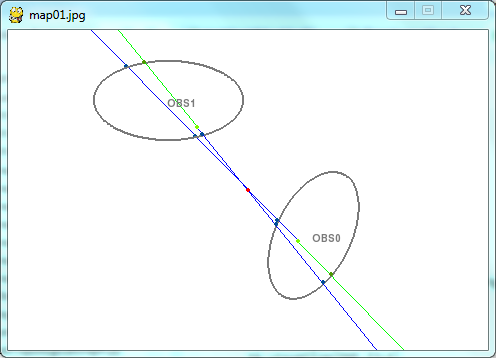
\includegraphics[width=\textwidth]{fig/obs_map.png}
		\caption{Decomposition of the map with obstacles.}
		\label{fig:obs_map:map}
	\end{subfigure}  
	%\\
	\begin{subfigure}[t]{0.5\linewidth}
		\centering
		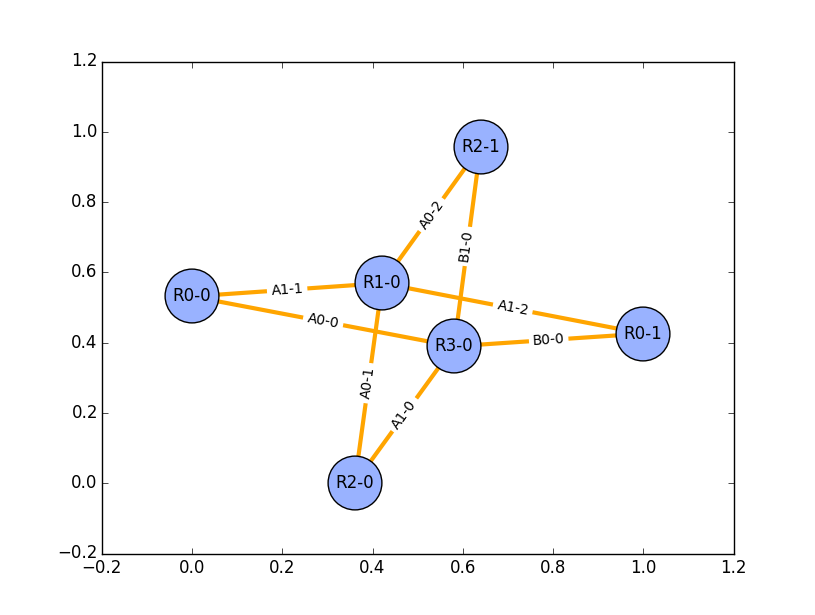
\includegraphics[width=\textwidth]{fig/obs_topology.png}
		\caption{The generated topological graph.}
		\label{fig:obs_map:topology}
	\end{subfigure}   
	\caption{Map with obstacles.}
	\label{fig:obs_map}
\end{figure}

We adopt the improved Jenkins' method in \cite{Hernandez201544} to generate reference frames given a map with obstacles.
The line segments, two ends of which connect with obstacles, are defined as \emph{reference frames}.
The reference frames decompose the map into several regions, which are the line segments formed by connecting the \emph{center point} $ c $ to a random \emph{obstacle point} $ b_{k} $ in each obstacle.
%{\sc This is ambiguous. Elaborate and use figure 1(a) to help describe how you form the line segments.}  
Given two paths, how they sequentially cross the reference frames can be used to identify homotopy equivalence.

%Observe how this process partitions the space $X$ into distinct regions, but note that the partition of $X$ differs from the partition of all possible paths through the space created by grouping paths into homotopic classes. 
%We use the partition of $X$ to identify a homotopic class as follows, again using the improved Jenkins' method.

Let $ \bm{B} $ denote the set of obstacles and $ B_{k} $ denote one of the obstacles.  
The generation of the reference frame is given in Algorithm \ref{alg:harrt:init_ref_frames}, which returns a set of reference frames $ \bm{R} $.
The called methods are explained as following,
\begin{itemize}
	\item \textsc{Line}($ p_{1}, p_{2} $):
	Return a line that defined by $ p_{1} $ and $ p_{2} $.
	\item \textsc{Ray}($ p, \vec{d} $):
	Return a ray that starts from $ p $ with direction $ \vec{d}  $.
	\item \textsc{Intersect}( $ r , \bm{B} $ ):
	Return line segments that a line $ r $ cut by the obstacles $ B $.
\end{itemize}
%{\sc What is B?}

Figure \ref{fig:obs_map:map} illustrates how the reference frames of a map is initialized.
$ b_{1} $ and $ b_{2} $ are randomly sampled from each obstacles.
Then a center point $ c $ is randomly sampled, which does not locate in any line connects any two $ b_{k} $.
For each $ b_{k} $, two rays are generated from two directions, $ \alpha_{k} $ is towards the center point $ c $, $ \beta_{k} $ is the reserved direction.
Both $ \alpha_{k} $ and $ \beta_{k} $ intersect with the obstacles $ B $, the line segment of which are the reference frames.
More details can be found in \cite{Hernandez201544}.

The reference frames can also be generated from a Voronoi diagram.
The improved Jenkin's method provides a much simpler initialization process in complex obstacles, especially in the regions adjacent to the map boundary.
It also avoids that the reference frames intersects with each other.
%As the reference frames are from the rays that rotate along the center point, the rotation order implies the direction of the path.

We can create a topological graph by the connectivity of the regions.
Each region from the map decomposition is a node in the topological graph.
Each reference frame is adjacent to two regions, thus it becomes an edge that connects two nodes.
Figure \ref{fig:obs_map:topology} shows a topological graph from the map decomposition in Figure \ref{fig:obs_map:map}.
%By the connectivity of the regions, we can generate a topological graph.  
%{\sc Explain how.  Essentially, each region in the partition of $X$ created by Jenkins' method is a vertex in the graph.  Edges between vertices are added between vertices if the vertices represent adjacent regions.}
%The nodes are the regions and the edges are the reference frames. 
%{\sc What do you mean "reference frame"?  This term hasn't been defined.}

Any path sequentially visits the regions maps to a node walk on the topological graph.
It is noticeable that two adjacent regions might be connected with not only one reference frame, which means that two nodes in the topological graph might be connected with more than one edge.
Thus, two path with same edge sequence belong to same homotopy class but two path with same node sequence don't.  
%Any path can be mapped into a sequence of nodes in the topological graph.  
%{\sc Explain how or given an example.}
%In determining the homotopy class, two paths share same start and goal.
%Thus they can be compared also by using only the visited edges, which are equivalent with the crossed reference frames. 
%{\sc Again, "reference frame" hasn't been adequately defined.  I believe it is the boundary between two regions.}
%Assign each reference frame a {\em character}. 
%{\sc Equivalently, assign each edge a character.}
%It is noticeable that the 
Label each reference frame with a \emph{character}.
Each path can be mapped into a {\em string}, which represents the sequence of the crossed reference frames.
In \cite{Hernandez201544}, the string is used to identify the homotopy class of each branch in RRT so that the growing of a tree is constrained in a homotopy class.
In this paper, each branch of the tree structure tracks the corresponding string as the homotopy information so that the homotopic constraints can be satisfied or the homotopy class can be identified.

%The string is used for the homotopy awareness in this paper, which inherits from \cite{Hernandez201544}.

%{\sc Do you explain how the string indicates the homotopy class?  
%The term ``homotopy awareness" is not defined adequately, and I suggest avoiding it.  

%Stating that some property of the algorithm ``inherits from [some reference]" doesn't explain to the reader %what you did. Are you just saying that we are describing how to algorithm in the reference works?  If so, say that instead of "inherits from."}

\begin{algorithm}[hbtp]
	\begin{algorithmic}[1]
		\State $ \bm{R} = \emptyset, \bm{b} = \emptyset, \bm{\alpha} = \emptyset, \bm{\beta} = \emptyset $
		\For{\textbf{each} $ B_{k} \in \bm{B} $ }
			\State $ b_{k} $ $ \leftarrow $ Randomly sample from $ B_{k} $
			\State $ \bm{b} \leftarrow \bm{b} \cup b_{k} $
		\EndFor
		\While{ $ \exists b_{k}, b_{k'} , c \in $ \Call{Line}{ $ b_{k}, b_{k'} $ } }
			\State $ c \leftarrow  $ Randomly sample from $ \bm{X}_{free} $
		\EndWhile
		\For{\textbf{each} $ b_{k} \in \bm{b} $ }
			\State $ \alpha_{k} \leftarrow $ \Call{Ray}{ $ b_{k}, c - b_{k} $ }
			\State $ \beta_{k} \leftarrow $ \Call{Ray}{ $ b_{k}, b_{k} - c $ }
			\State $ \bm{\alpha} \leftarrow \bm{\alpha} \cup \alpha_{k} $
			\State $ \bm{\beta} \leftarrow \bm{\beta} \cup \beta_{k} $			
		\EndFor
		\For{\textbf{each} $ \alpha_{k} \in \bm{\alpha} $}
			\State $ \{ \alpha_{k_{m}} \} \leftarrow $ \Call{Intersect}{$ \alpha_{k}, \bm{B} $}
			\State $ \bm{R} \leftarrow \bm{R} \cup \{ \alpha_{k_{m}} \} $
		\EndFor
		\For{\textbf{each} $ \beta_{k} \in \bm{\beta} $}
			\State $ \{ \beta_{k_{m}} \} \leftarrow $ \Call{Intersect}{$ \beta_{k}, \bm{B} $}
			\State $ \bm{R} \leftarrow \bm{R} \cup \{ \beta_{k_{m}} \} $
		\EndFor
		\Return $ \bm{R} $
	\end{algorithmic}
	\caption{ \textsc{InitRefFrames} ($ \bm{X}_{free} , \bm{B} $) }
	\label{alg:harrt:init_ref_frames}
\end{algorithm} 

With the generated reference frames $ \mathbf{R} $, we could import the bidirectional RRT$^{*}$ to accomplish the homotopy-aware exploration process.
We notice that two string can be generated from two paths that belongs to same homotopy class.
We define the \emph{homotopic grammar} to determine whether two string belongs to same homotopy class.


%{\sc So, is $\mathbf{R}$ the set of unique characters assigned to the edges of your graph? Is $\mathbf{B}$ the set of regions in the world, so each $B_k \in \mathbf{B}$ is a region?}

%{\sc How is $c$ sampled in line 6? What is $\mathbf{b}$ and how is it initialized -- line 4.}

The process is given in Algorithm \ref{alg:harrt}.
Two trees, the \emph{start tree} $ G_{s} $ and the \emph{goal tree} $ G_{g} $, are constructed from $ x_{init} $ and $ x_{goal} $ respectively.
Two trees explore the map bidirectionally by calling {\sc Explore}(), defined in Algorithm \ref{alg:harrt:explore}, at each iteration.
By using each new vertex returned from {\sc Explore}(), we can call {\sc Connect}() to create a path with a vertex in the other tree.
The created path will be compared with the current best path that belongs to the same homotopy class.
If it is a better one, the best path in this homotopy class will be updated, which is implemented in {\sc UpdateBestPathByClass}().

\begin{algorithm}[hbtp]
	\begin{algorithmic}[1]
		\State $ i \leftarrow 0 $
		\State $ V_{s} \leftarrow \{ x_{init} \} $; $ E_{s} \leftarrow \emptyset $; $ G_{s} \leftarrow (V_{s}, E_{s}) $
		\State $ V_{g} \leftarrow \{ x_{goal} \} $; $ E_{g} \leftarrow \emptyset $; $ G_{g} \leftarrow (V_{g}, E_{g}) $
		\While{ $ i < N $ }
			\State $ G_{s}, x_{s}^{new} \leftarrow $ \Call{Explore}{$ G_{s}, i $}
			\State $ G_{g}, , x_{g}^{new} \leftarrow $ \Call{Explore}{$ G_{g}, i $}
			\State $ p_{s} \leftarrow $ \Call{Connect}{$  x_{s}^{new}, G_{g} $}
			\State $ p_{g} \leftarrow $ \Call{Connect}{$  x_{g}^{new}, G_{s} $}
			\State $ P \leftarrow $ \Call{UpdateBestPathByClass}{$ p_{s}, P $}
			\State $ P \leftarrow $ \Call{UpdateBestPathByClass}{$ p_{g}, P $}
			\State $ i \leftarrow i + 1 $
		\EndWhile
		\State $ P \leftarrow $ \Call{MergePaths}{$ P $}
		\Return $ P $
	\end{algorithmic}
	\caption{HA-RRT$^{*}$ ($ x_{init} , x_{goal} $) }
	\label{alg:harrt}
\end{algorithm}


\begin{algorithm}[hbtp]
	\begin{algorithmic}[1]
		\State $ x_{rand} \leftarrow $ \Call{ Sample }{$ i $} ;
		\State $ x_{nearest} \leftarrow $ \Call{Nearest}{$ G, x_{rand} $}
		\State $ x_{new} \leftarrow $ \Call{Steer}{$ x_{nearest}, x_{rand},\eta $}
		\If{ \Call{ObstacleFree}{$ x_{nearest}, x_{new} $} }
			%\State $ G \leftarrow $ \Call{ Extend }{$ G, x_{new}, x_{\it nearest} $}
			\State $ x_{min} \leftarrow x_{nearest} $
			\State $ X_{near} \leftarrow $ \Call{Near}{$ G, x_{new}, | V | $}
			\State $ s \leftarrow $ \Call{STR}{$x_{new}$} $ \cup $ \Call{CRF}{$ ( x_{new}, x_{near} ), \bm{B} $}
			\If{\Call{HomotopyCheck}{$ s $}}
				\For{\textbf{each} $ x_{near} \in X_{near} $ }
					\If{ \Call{ObstacleFree}{$ x_{new} , x_{near} $} }
						\If{ \Call{Cost}{$ x_{near} $} $ + c( $ \Call{Line}{$ x_{near}, x_{new} $} $ ) < $ \Call{Cost}{$ x_{new} $} } 
							\State $ x_{min} \leftarrow x_{near} $
						\EndIf
					\EndIf
				\EndFor

				\State $ E' \leftarrow E' \cup \{ ( x_{min}, x_{new} ) \} $
				\For{\textbf{each} $ x_{near} \in X_{near} \setminus \{ x_{min} \} $ }
					\If{\Call{ObstacleFree}{$ x_{new} , x_{near} $} and \Call{Cost}{$ x_{near} $} $ > $ \Call{Cost}{$ x_{new} $} + c(\Call{Line}{$ x_{new}, x_{near} $}) }
					   \State $ s \leftarrow $ \Call{STR}{$x_{new}$} $ \cup $ \Call{CRF}{$ ( x_{new}, x_{near} ), \bm{B} $}
					   \If{\Call{HomotopyCheck}{$ s $}}
					   		\State $ x_{parent} \leftarrow $ \Call{Parent}{$ x_{near} $}
							\State $ E' \leftarrow E' \setminus \{ ( x_{parent}, x_{near} ) \} $
							\State $ E' \leftarrow E' \cup \{ ( x_{new}, x_{near} ) \} $
					   \EndIf
					\EndIf
				\EndFor	
			\EndIf
		\EndIf
		\Return $ G, x_{new} $
	\end{algorithmic}
	\caption{ \textsc{Explore}($ G, i $) }
	\label{alg:harrt:explore}
\end{algorithm}

The {\sc Explore} procedure is inherited from the process in \cite{Karaman-RSS-10}.
In the {\sc Explore} procedure, the {\sc HomotopyCheck}() uses a state machine to check whether the string satisfies the defined grammar.
The called methods are defined as following:
\begin{itemize}
	\item \textsc{CRF}($ l, \bm{R} $):
	Returns the character that represents the crossed reference frames if any.
	\item \textsc{STR}($ x $):	
	Returns the string that represents the crossed reference frames sequentially.
	%\item \textsc{HomotopyCheck}{($ s $)}
	%Returns if the path or subpath $ s $ satisfies a given homotopy constraint.
\end{itemize}

The {\sc HomotopyCheck}() guarantees that adding new edge or rewiring edges all satisfies the homotopy constraint. {\sc How?}
The homotopy constraint is defined as a \emph{homotopic grammar}.
{\sc New concept.  You need to introduce a concept and explain something about it before you use it, or you must tell the reader what purpose the concept serves {\bf and} that you will explain it later in the paper.}
Because RRT$^{*}$ maintains a tree structure, each vertex has only one path to arrive from the root.
This path, which starts from the root to the vertex, indicates a string of characters sequentially.
Each character represents a crossed reference frame. 
{\sc Need to explain  this better.}

The {\sc Connect} procedure connects a vertex with the other tree to generate a path from the start to goal.
In order to guarantee optimality, a set of near vertices is provided to find the best vertex to be connected with.
The methods in Algorithm \ref{alg:harrt:binding} are defined as following:
\begin{itemize}
	\item \textsc{Path}($ v, G $):	
	Returns the path from the root of $ G $ to the vertex $ v $.
	\item \textsc{Concatenate}{($ p_{a}, p_{b} $)}
	Returns a concatenated path of $ p_{a} $ and $  p_{b} $.
	If $ p_{a} $ and $  p_{b} $ are from different directions, one of the them will be reversed for the concatenation.
\end{itemize}

\begin{algorithm}[hbtp]
	\begin{algorithmic}[1]
		\State $ p_{min} = \emptyset $
		\State $ X_{near} \leftarrow $ \Call{NEAR}{$ G, x_{new}, |V| $}
		\For{\textbf{each} $ x_{near} \in X_{near} $ }
		    \If{ \Call{ObstacleFree}{$ x_{new}, x_{near} $} } 
			    \If{ $ x_{new} \in G_{s} $ }
					\State $ p \leftarrow $ \Call{Concatenate}{$  x_{new} ,  x_{near} $}
				\Else
				    \State $ p \leftarrow $ \Call{Concatenate}{$  x_{near}, x_{new} $}			
				\EndIf
			    \If{ \Call{HomotopyCheck}{$ p $} and $ c( p ) < c( p_{min} ) $ }
			    	\State $ p_{min} = p $
			    \EndIf 
			\EndIf
		\EndFor
		\Return $ p_{min} $
	\end{algorithmic}
	\caption{ \textsc{Connect}($ x_{new}, G $) }
	\label{alg:harrt:binding}
\end{algorithm}

Because both the start tree $ G_{s} $ and the goal tree $ G_{g} $ add a new vertex. 
The {\sc Connect} procedure creates a path by connecting the new vertex with the other tree, which are $ p_{s} $ and $ p_{g} $ correspondingly.
The new paths will be used to update the best path of the homotopy classes they belong to in {\sc UpdateBestPathByClass} ().

When the exploration process is finished, there is a set that contains the best paths for all the homotopy classes.
Because the homotopy class is defined by the string,
there exist different strings belong to same homotopy classes.
The {\sc MergePaths} procedure will be called to merge the equivalent homotopy classes. 
Thus the set of paths $ P $ will be updated.

\section{Homotopy-aware optimal path planning}
\label{sec:application}

By the homotopy-aware exploration process, HA-RRT$^{*}$ can return optimal path with given homotopy constraints.
In this section, we show the sliding autonomy in different levels of the human's intent on the topology by using HA-RRT$^{*}$.

\subsection{Homotopic constraint from a reference path}

In planning a path for a task, if the human has a determined mind of how the topology of the path should be, the HA-RRT$^{*}$ can help to find the optimal path in all the paths of a given topology.
By an interactive process, the human can initialize a reference path to represent the topology from his/her intent.

\begin{figure}
	\centering
	\begin{subfigure}[t]{0.47\linewidth}
		\centering
		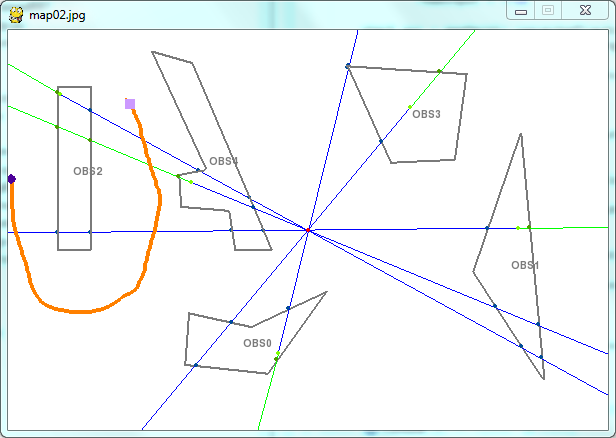
\includegraphics[width=\textwidth]{fig/referenceHomotopy.png}
		\caption{Reference path}
		\label{fig:reference_path:reference}
	\end{subfigure}  
	%\\
	\begin{subfigure}[t]{0.47\linewidth}
		\centering
		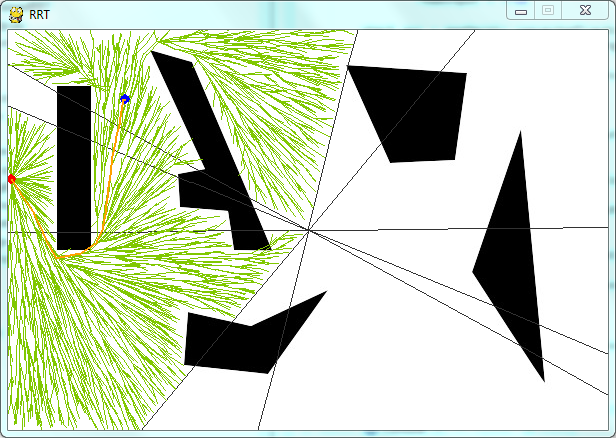
\includegraphics[width=\textwidth]{fig/homotopicConstrainedRRT.png}
		\caption{RRT$^{*}$ with homotopic constraint}
		\label{fig:reference_path:rrt}
	\end{subfigure}   
	\caption{Homotopic constraint from a reference path.}
	\label{fig:reference_path}
\end{figure}

Figure \ref{fig:reference_path} gives an example.
A user firstly initializes a reference path, which indicates the intended homotopy class as in Figure \ref{fig:reference_path:reference}.
The string of the reference path is then extracted as the constraint.
The exploration of HA-RRT$^{*}$ is then under this constraint.
Thus, in Figure \ref{fig:reference_path:rrt}, the tree only explores the regions that does not violate the grammar to generate the constraint string.

\subsection{Homotopic constraints from required/forbidden regions}

In planning a path for a task, if the human only can tell several regions that should be avoided or several regions that are required to visit, HA-RRT$^{*}$ explores the paths that satisfies the defined constraints as well.
The {\sc InitRefFrames} procedure decomposes the map and generates the topological graph, for which Figure \ref{fig:obs_map:map} gives an example.
We define the \emph{positive region} as the region that is required to visit and the \emph{negative region} as the region that is forbidden to visit.
Then there is an interactive process for the human to label the positive regions and the negative regions.
Unlabeled regions are neutral, which means no constraint here.
Figure \ref{fig:region_label} shows an example.
By defining the positive region and the negative region in Figure \ref{fig:region_label:label}, in which the red region indicates the negative region and the green region indicates the positive region.
The homotopy classes that satisfy the constraint can be obtained by traversing the topological graph, which is illustrated in Figure \ref{fig:region_label:constraint}.

Because the decomposed regions are randomly and automatically generated, a decomposed region might contain both positive regions and negative regions.
In this case, the decomposed region will be split into several smaller regions so that each region might contain either positive region or negative region.
After that, more reference frames will be created correspondingly and a new topological graph will be obtained.

\begin{figure}
	\centering
	\begin{subfigure}[t]{0.47\linewidth}
		\centering
		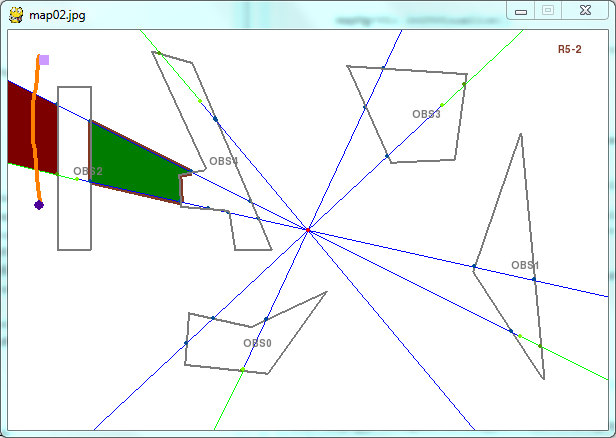
\includegraphics[width=\textwidth]{fig/regionlabel1.png}
		\caption{Labeling the regions}
		\label{fig:region_label:label}
	\end{subfigure}  
	%\\
	\begin{subfigure}[t]{0.47\linewidth}
		\centering
		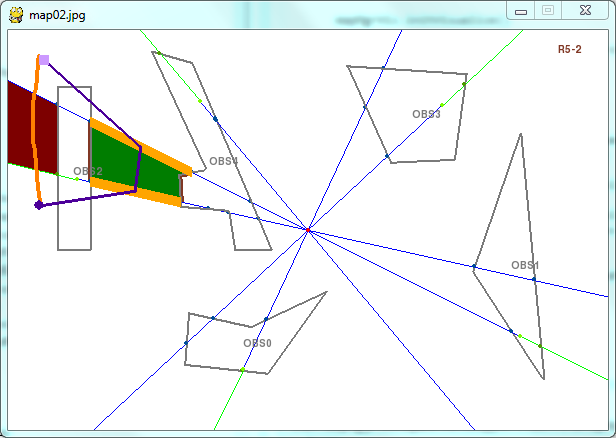
\includegraphics[width=\textwidth]{fig/regionlabelhomo1.png}
		\caption{Homotopy class satisfies the labeled regions}
		\label{fig:region_label:constraint}
	\end{subfigure}   
	\caption{Labeling region to generate homotopic constraints.}
	\label{fig:region_label}
\end{figure}

As each region is a node in the topological graph, the nodes of the negative regions can be trimmed firstly.
A breath first search on the topological graph can return a set of strings that satisfy the labeled constraints, which also indicates a set of homotopy classes. nb
The grammar is then defined by this set of strings.
The {\sc HomotopyCheck} in the exploration of HA-RRT$^{*}$ will be defined by this grammar.
The path returned by the HA-RRT$^{*}$ is the optimal solution under the labeled constraint.

\subsection{Homotopy classes with preference}

Sometimes there exists no hard constraint on the topology of the paths.
But there does exist the difference on different topology.
For example, visiting some region benefits some sub-task, or going around some object enhances the task performance.
If the human can tell the preference on the topology, scores can be assigned to each homotopy class.

Consider the topology as a discrete variable, the values of the variable is the set of all the homotopy classes.
The problem can be viewed as a two-objective optimization problem.
Figure \ref{fig:all_homotopy:no_pref} provides an example of the optimal paths in four homotopy classes.
Because the optimal solution in one homotopy class dominates all other solutions in the same class.
By combining the optimal paths in all the homotopy classes, we can find the non-dominated paths from them.
Figure \ref{fig:homotopy_human_interaction:pareto_score} illustrates such a Pareto front.

\begin{figure}
	\centering
	\begin{subfigure}[t]{0.47\linewidth}
		\centering
		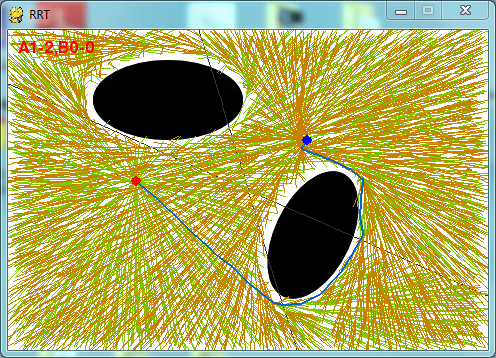
\includegraphics[width=\textwidth]{fig/all_homotopy1.png}
		\caption{Best path in one homotopy class.}
		\label{fig:all_homotopy:01}
	\end{subfigure}  
	%\\
	\begin{subfigure}[t]{0.47\linewidth}
		\centering
		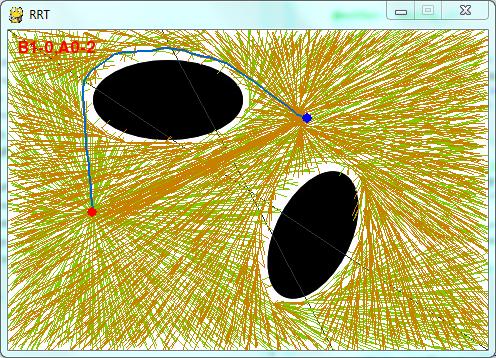
\includegraphics[width=\textwidth]{fig/all_homotopy2.png}
		\caption{Best path in one homotopy class.}
		\label{fig:all_homotopy:02}
	\end{subfigure}
	\\
	\begin{subfigure}[t]{0.47\linewidth}
		\centering
		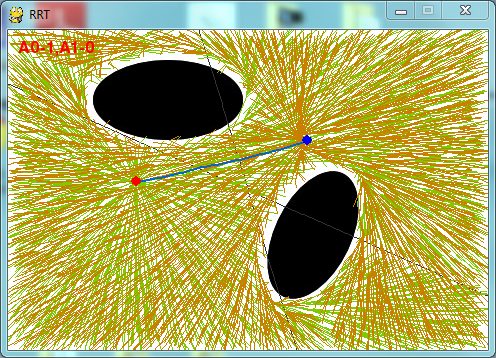
\includegraphics[width=\textwidth]{fig/all_homotopy3.png}
		\caption{Best path in one homotopy class.}
		\label{fig:all_homotopy:03}
	\end{subfigure}  
	%\\
	\begin{subfigure}[t]{0.47\linewidth}
		\centering
		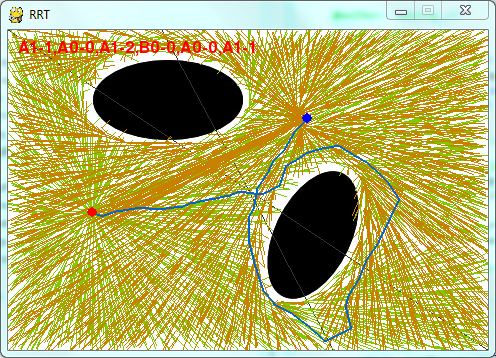
\includegraphics[width=\textwidth]{fig/all_homotopy4.png}
		\caption{Best path in one homotopy class.}
		\label{fig:all_homotopy:all_scores}
	\end{subfigure}	   
	\caption{Bidirectional RRT$^{*}$.}
	\label{fig:all_homotopy:no_pref}
\end{figure}

\subsection{Homotopy classes without preference}

Sometimes inherently the user has a mind of the topology preference but is too fuzzy to describe.
If the topology is included to have a two-objective optimization problem, it means that the optimal paths in all the homotopy classes are non-dominant.
Thus HA-RRT$^{*}$ will show the optimal paths of all the homotopy classes.
Figure \ref{fig:homotopy_human_interaction:all_scores} gives an example of the scores.
With the interface of visualizing the optimal path in different homotopy class, the human can select one from them that matches his intent most.

\begin{figure}
	\centering
	\begin{subfigure}[t]{0.47\linewidth}
		\centering
		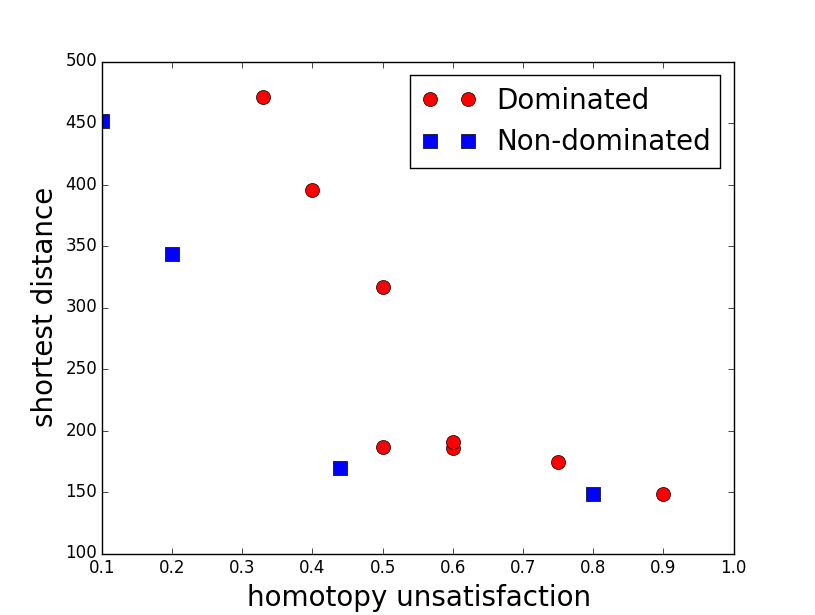
\includegraphics[width=\textwidth]{fig/pareto_score.png}
		\caption{Pareto front with topology preference.}
		\label{fig:homotopy_human_interaction:pareto_score}
	\end{subfigure}  
	%\\
	\begin{subfigure}[t]{0.47\linewidth}
		\centering
		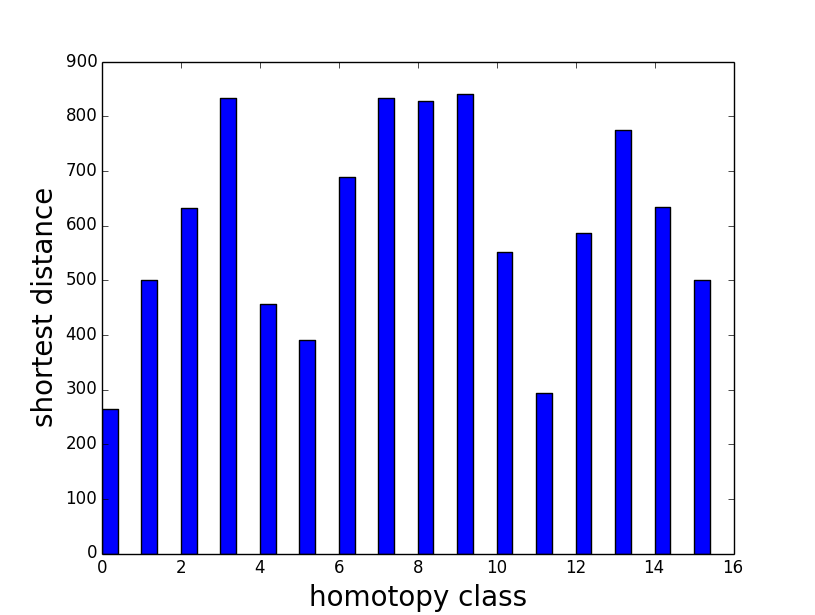
\includegraphics[width=\textwidth]{fig/all_homotopy_score.png}
		\caption{Minimum cost in all the homotopy classes.}
		\label{fig:homotopy_human_interaction:all_scores}
	\end{subfigure}   
	\caption{Interactive optimization.}
	\label{fig:homotopy_human_interaction}
\end{figure}


\section{Analysis}
\label{sec:analysis}

The HA-RRT$^{*}$ consists of the homotopy-aware exploration and the constrained optimization.
In this section, we look at how to have better support on the homotopy classes and provide the constrained optimal guarantee.

\subsection{homotopic grammar}

Because each path or subpath can be converted into a string, which represents a sequence of characters by crossed reference frames.
When we have a set of homotopy classes, a homotopic grammar can be created to define all the strings of the set of homotopy classes.
The homotopic grammar is used to manage the exploration process in {\sc HomotopyCheck} and determine which homotopy class a path belongs to by its string.

\begin{figure}
	\centering
	\begin{subfigure}[t]{0.4\linewidth}
		\centering
		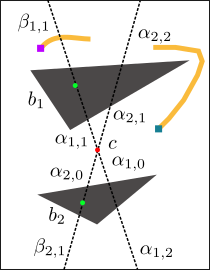
\includegraphics[width=\textwidth]{fig/feasibility}
		\caption{Feasibility}
		\label{fig:grammar:feasibility}
	\end{subfigure}  
	\begin{subfigure}[t]{0.4\linewidth}
		\centering
		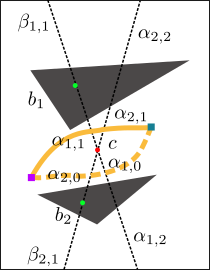
\includegraphics[width=\textwidth]{fig/equivalence}
		\caption{Equivalence}
		\label{fig:grammar:equivalence}
	\end{subfigure}
	\\
	\begin{subfigure}[t]{0.4\linewidth}
		\centering
		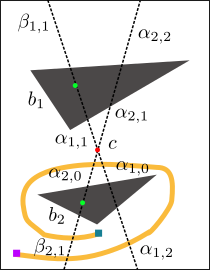
\includegraphics[width=\textwidth]{fig/recurring}
		\caption{Recurring}
		\label{fig:grammar:recurring}
	\end{subfigure}  
	\begin{subfigure}[t]{0.4\linewidth}
		\centering
		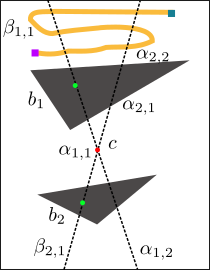
\includegraphics[width=\textwidth]{fig/repeated_pattern}
		\caption{Equivalence}
		\label{fig:grammar:repeated_pattern}
	\end{subfigure} 
	\caption{Homotopic grammar.}
	\label{fig:grammar}
\end{figure}

There are several properties in the homotopic grammar which indicates some information of the paths.
\begin{itemize}
\item \textbf{Feasibility}
As the reference frames are connected by the regions, any strings from the grammar must be a feasible one.
A feasible string means that any two sequential characters of it are connected in the topological graph by the nodes of the regions.
An example is given in Figure \ref{fig:grammar:feasibility}.

\item \textbf{Equivalence}
Some characters of the reference frames are equivalent in constructing the strings.
All the reference frames contains the center point $ c $ show this property.
The segment crossing those reference frames in any sequence belongs to same homotopy class.
Figure \ref{fig:grammar:equivalence} shows an example.

\item \textbf{Recurring character}
Recurring character in a string indicates that the path goes around some obstacles and back to a visited region.
Recurring equivalent characters also has same effect.
One example is illustrated in Figure \ref{fig:grammar:recurring}.

\item \textbf{Repeated pattern}
Repeated pattern shows that the path is back and forth among some regions.
In minimization problem, it is not useful and can be often ignored.
Because repated pattern will only increase the cost if the cost function is additive.
However, in some special scenario, for example it is expected to scan a region for a fixed number of times, the repeated pattern can be used.

\end{itemize}

\subsection{Optimality with constraint}

The way that the RRT$^{*}$ algorithm works is that it incrementally constructs a tree from a root position.  
The cost of the path from the position of the root node to the positions of every other node converges to the minimal possible cost between the positions as the number of iterations approaches infinity.  
We restate this as a lemma, and note that the corresponds exactly to that given for Theorem 22 in~\cite{Karaman-RSS-10}.
\begin{lem}
\label{lem:tree_vex:conv}
Given Assumptions 1 - 3 in \cite{Karaman-RSS-10},
the cost of the minimum cost path from the root to any vertex in RRT$^{*}$ converges to the optimal cost almost surely.
\end{lem}

HA-RRT$^{*}$ uses bidirectional trees to explore the workspace.
In {\sc Connect} procedure, the vertex $ v $ in either $ G_{s} $ or $ G_{g} $ is used to create a path by connecting with another vertex in the other tree.
If we see the position of $ v $ as a via-point of the paths, we can have the asymptotic optimality with the set of paths has $ v $ as via-point.
It is stated in Lemma \ref{lem:optimal_via_point}.

\begin{lem}
\label{lem:optimal_via_point}
Given Assumptions 1 - 3 in \cite{Karaman-RSS-10},
the path concatenated from a path from $ G_{s} $ for $ v $ and a path from $ G_{g} $ for $ v $ converges to the optimal path through $ v $ almost surely. 

\begin{proof}
Look at connecting a vertex $ v_{s} $ in $ G_{s} $ with the $ G_{g} $.
Let $ c (v_{s}) $ denote the cost of the $  v_{s}  $ in $ G_{s} $, which is the cost-to-come from the start to the position of $  v_{s} $.
Let $ v_{g} $ be the vertex to be connected in $ G_{g} $.
Let $ c ( v_{g} ) $ denote the cost of the $  v_{g} $ in $ G_{g} $, which is the cost-to-come from the goal to the position of $  v_{g} $.
It equals to the cost-to-go from the position of $ v_{g} $ to the goal.
Let $ \sigma_{G_{s},G_{g}} (v_{s}, v_{g}) $ be a path concatenated by two sub-paths from $  v_{s} $ and $  v_{g} $. 
Its cost $ {\sc Cost} (\sigma_{G_{s},G_{g}} ( v_{s}, v_{g} )) =  c (v_{s}) + c (v_{g}) + c (${\sc Line}$ (v_{s}, v_{g})  ) $.
By Lemma \ref{lem:tree_vex:conv}, we know that $ c (v_{s}) $ and $ c (v_{g}) $ converge to optimal almost surely.
$ c (${\sc Line}$ (v_{s}, v_{g})  ) $ will also converge, because $ v_{g} $ is selected from a set of near vertices.
Thus, the cost of $ \sigma_{G_{s},G_{g}} (v_{s}, v_{g}) $ converges to optimal almost surely. 
Similarly, we can have the same result on connecting a vertex $ v_{g} $ in $ G_{g} $ with the $ G_{s} $.
\end{proof}
\end{lem}

By Lemma \ref{lem:optimal_via_point} we can have Theorem \ref{thm:constrained_optimality} and Theorem \ref{thm:homotopy_pref:optimal}.
Theorem \ref{thm:constrained_optimality} and Theorem \ref{thm:homotopy_pref:optimal} guarantees that the applications mentioned in Section \ref{sec:application} can find the optimal solutions as stated.

\begin{thm}
\label{thm:constrained_optimality}
Given Assumptions 1 - 3 in \cite{Karaman-RSS-10},
HA-RRT$^{*}$ can find the optimal path in one homotopy class almost surely.
\end{thm}

\begin{thm}
\label{thm:homotopy_pref:optimal}
Given Assumptions 1 - 3 in \cite{Karaman-RSS-10}, 
HA-RRT$^{*}$ can find all the non-dominated paths when the topology is an objective.
\end{thm}


\subsection{Discussion}

When the homotopy classes are used as the constraint, one directional RRT$^{*}$ can also find the optimal path.
It is only a constrained optimization problem.
The bidirectional RRT$^{*}$ accelerates the convergence rate, like in \cite{starek2014bidirectional}.
When the homotopy classes are used more than only the constraint, bidirectional RRT$^{*}$ is required so that each position can have the optimal-to-come sub-path and optimal-to-go sub-path.
In this way, we can have the optimal path in each homotopy class.

\begin{comment}
In the bidirectional exploration, the two direction can share the same workspace or split the workspace.
Figure \ref{fig:homotopy_no_pref} provides two cases.
In Figure \ref{fig:homotopy_no_pref:all}, both two trees parallel explore on the same workspace.
While in Figure \ref{fig:homotopy_no_pref:half}, the workspace has been split into two.
Each tree explores only explore half ot the workspace it is in.
Theoretically, HA-RRT$^{*}$ converge to have same solutions in both two cases.
In most of the case, splitting the workspace makes better efficiency, especially there are less vertices belong to both two trees.
However, the convergence rate depends on the convergence of the vertices near the boundary in both two trees.
\end{comment}

As we noticed, with a topological graph, it is possible that several strings belong to same homotopy class.
Thus, the string equivalence on the homotopy class should be considered.
Because of the property of the repeated pattern, determining the strings in one homotopy class increases the algorithm complexity.
In a minimization problem, assuming the path length is always relevant with the total cost, it is fair to forbid the properties of recurring and repeated pattern.
In this way, a breath first search can return all the possible strings from the topological graph.
Thus the efficiency can be enhanced.
However, the flexibility in supporting more types of paths is lost.
In application, the trade-off between the efficiency and the topology versatility should be considered by case.

\section{Conclusion}
\label{sec:conclusion}

In this paper, we propose a homotopy-aware RRT$^{*}$, which tracks the homotopy class each branch belongs to.
By using a bidirectional structure, the asymptotic optimality in each homotopy class can also be guaranteed.
This enables the sliding autonomy to support different level of task supervisor's intent on the topology in planning paths.
The way of communication is also more natural for the human, because the human can directly visualize the path ``shape'' instead of converting to the robot's data format.
It also supports the application of more complicated tasks, especially when there is requirement on the topology of the paths in a complex map.
The homotopy-aware RRT$^{*}$ can be introduced to the multi-objective optimization to cover the increasing complexity of the tasks to the robots.
Also an online identification of the human's intent might start the workspace reduction earlier so that the efficiency could be enhanced.

\bibliographystyle{IEEEtranS}
\bibliography{reference}

\end{document}